\documentclass[11pt,a4paper]{article}

% ---------------------------------------------------------------------------
% Packages (deliberately limited to widely available, reliable packages)
% ---------------------------------------------------------------------------
\usepackage[T1]{fontenc}
\usepackage[utf8]{inputenc}
\usepackage[htt]{hyphenat}
\usepackage[a4paper,margin=2.4cm]{geometry}
\usepackage{graphicx}
\usepackage{subcaption}
\usepackage{booktabs}
\usepackage{longtable}
\usepackage{tabularx}
\usepackage{array}
\usepackage{enumitem}
\usepackage{caption}
\usepackage{float}
\usepackage{xcolor}
\usepackage[hidelinks]{hyperref}
\usepackage{url}

\graphicspath{{figures/}}
\captionsetup{font=small,labelfont=bf}
\setlist{topsep=2pt,itemsep=1pt,parsep=0pt}
\newcolumntype{L}[1]{>{\raggedright\arraybackslash}p{#1}}
\newcommand{\code}[1]{\texttt{#1}}

\title{\textbf{Comparative Analysis and Suitability Assessment of Two\\Transactional Datasets for a Governed Multi-Agent\\E-Commerce and Accounting System}}
\author{Research Engineer / Data Scientist\\\small Governed Multi-Agent AI for Autonomous E-Commerce and Accounting Operations}
\date{\today}

\begin{document}

% ===========================================================================
% TITLE PAGE
% ===========================================================================
\begin{titlepage}
\centering
\vspace*{1.5cm}
{\Huge\bfseries Dataset Analysis and Suitability Report\par}
\vspace{0.6cm}
{\Large Comparative Analysis of the Olist Brazilian E-Commerce Dataset\\[2pt] and the Online Retail II Dataset\par}
\vspace{1.2cm}
{\large For the project\par}
\vspace{0.3cm}
{\Large\itshape Governed Multi-Agent AI for Autonomous\\E-Commerce and Accounting Operations\par}
\vspace{2.0cm}
\vfill
\begin{tabular}{rl}

\textbf{Document type:} & Dataset analysis and recommendation report \\[4pt]
\textbf{Analysed datasets:} & Olist Brazilian E-Commerce Public Dataset \\
 & Online Retail II (UCI Machine Learning Repository) \\[4pt]
\textbf{Analysis artefacts:} & \code{analysis/}, \code{analysis\_results/}, \code{figures/} \\[4pt]
\textbf{Date:} & \today \\
\end{tabular}
\vfill
{\small All numerical results in this report were computed from the local copies of the datasets by the accompanying analysis package; no values were fabricated. Where a capability is absent from the data, this is stated explicitly.}
\end{titlepage}

% ===========================================================================
% ABSTRACT
% ===========================================================================
\begin{abstract}
\noindent
This report analyses two real, independent transactional datasets --- the Olist Brazilian E-Commerce Public Dataset (nine relational CSV files) and the Online Retail II dataset (one Excel workbook with two annual worksheets) --- in order to assess their suitability as evidence sources for a proposed governed multi-agent system covering e-commerce operations, accounting-related workflows, anomaly detection and auditability. Using a reproducible Python package, we profiled every file and sheet, measured missingness, duplicates, cardinality, temporal coverage, candidate keys, referential integrity and join behaviour, and derived a small number of transparent business and data-quality signals. The Olist dataset contains 1,550,922 rows over nine tables with a normalised schema and clean key relationships, but exhibits no stock, ledger or policy information and has notable duplicate geolocation rows (26.18\%). Online Retail II contains 1,067,371 invoice lines with no relational structure, but supports transaction-level revenue, cancellation and customer analysis, at the cost of 22.77\% missing customer identifiers and several data-quality signals (negative quantities, zero/negative prices, cancellations). We conclude that Olist is the stronger \emph{primary} source for multi-table e-commerce workflows and auditing experiments, while Online Retail II is a useful \emph{complementary} transaction-level source. Neither dataset implements a multi-agent system, contains native governance policies, ground-truth fraud labels, a general ledger, or inventory stock levels. We therefore specify a prototype-based experimental plan, an audit event schema and an evaluation protocol, and we clearly separate measured results from proposed methods and expected outcomes.
\end{abstract}

\tableofcontents
\clearpage

% ===========================================================================
\section{Introduction and Research Context}
% ===========================================================================
The project \emph{Governed Multi-Agent AI for Autonomous E-Commerce and Accounting Operations} investigates how a set of specialised, governed software agents can cooperate to perform e-commerce and accounting workflows while remaining traceable and auditable. The intended agent roles are: an Orchestrator/Coordination agent; an E-Commerce agent; an Inventory agent; an Accounting agent; a Risk/Anomaly-Detection agent; a Governance agent; and an Audit agent.

The research requires concrete, real-world data to (i) ground the workflows in plausible business records, (ii) design validation, reconciliation and anomaly-detection rules, and (iii) evaluate the prototype. This report examines two publicly available datasets and answers three questions:

\begin{enumerate}[label=(\roman*)]
\item What do the datasets actually contain, and what is their quality?
\item How suitable is each dataset for each proposed agent, and for governance and audit experiments?
\item Which dataset should be the primary source, which the complementary source, and under what conditions?
\end{enumerate}

\paragraph{Scope and integrity statement.}
The datasets are treated strictly as \emph{evidence sources}. They are records of business transactions; they do not implement agents, do not contain governance policies, and do not provide ground-truth labels for fraud. Throughout this report, observations (measured from the data) are distinguished from interpretations and from proposals for future work. All numbers were produced by the accompanying analysis package running against the local files, and are reproduced in machine-readable form under \code{analysis\_results/}.

% ===========================================================================
\section{Research Objectives and Dataset Selection Criteria}
% ===========================================================================
The dataset evaluation is guided by the following criteria, derived from the agent roles and from the project's governance and audit objectives:

\begin{itemize}
\item \textbf{Business coverage:} does the data describe orders, payments, products, sellers and customers?
\item \textbf{Relational structure:} are entities linked through keys so that multi-step, cross-entity workflows can be constructed and validated?
\item \textbf{Accounting relevance:} are monetary amounts present at transaction and order level, with enough consistency to prototype reconciliation?
\item \textbf{Anomaly-detection potential:} are there numeric distributions, temporal sequences and integrity constraints from which candidate anomalies can be derived?
\item \textbf{Auditability:} can every agent decision be traced back to identifiable source records?
\item \textbf{Data quality:} missingness, duplicates and key integrity.
\item \textbf{Licensing and reproducibility:} can the data be used and the analysis reproduced under clear terms?
\end{itemize}

Two real datasets were located in the project directory and used. No synthetic or merged data were employed.

% ===========================================================================
\section{Dataset Sources and Descriptions}
% ===========================================================================
\subsection*{Dataset 1 --- Olist Brazilian E-Commerce Public Dataset}
Olist is a Brazilian marketplace operator. The public dataset, distributed on Kaggle, contains anonymised order data from approximately 100{,}000 orders placed between 2016 and 2018 across multiple marketplaces, together with customer location, product attributes, payment, review and geolocation information \cite{olistDataset}. In the local copy, the dataset is stored as nine CSV files in \code{datasets/olist/}. The Kaggle data card states the licence as \textbf{CC BY-NC-SA 4.0} (attribution, non-commercial, share-alike), which constrains redistribution and commercial reuse; this must be re-checked against the current data card before any publication or sharing of raw data. Monetary amounts are in Brazilian Reais (BRL).

\subsection*{Dataset 2 --- Online Retail II}
Online Retail II is an UCI Machine Learning Repository dataset donated by Daqing Chen \cite{chen2012}. It records all transactions of a UK-based, registered, non-store online retailer selling gift-ware, mostly to wholesalers, between 1 December 2009 and 9 December 2011. The official record reports 1{,}067{,}371 instances and licenses the data under \textbf{CC BY 4.0} (Creative Commons Attribution 4.0 International), which permits sharing and adaptation with attribution. The local copy is a single Excel workbook \code{datasets/online\_retail\_ii/online\_retail\_II.xlsx} with two worksheets, \code{Year 2009-2010} and \code{Year 2010-2011}. Monetary amounts are in pounds sterling (\pounds).

\paragraph{Provenance verification.} The UCI record (creator, DOI \code{10.24432/C5CG6D}, licence CC BY 4.0, instance count and date range) was verified directly from the UCI web page during preparation. The Olist Kaggle data card (title, provider, nine-file listing, licence CC BY-NC-SA 4.0) was verified from the Kaggle listing.

% ===========================================================================
\section{Methodology for Dataset Inspection}
% ===========================================================================
\subsection{Reproducible analysis package}
All results were produced by a small Python package (\code{analysis/}) using \code{pandas}, \code{NumPy}, \code{matplotlib}, \code{seaborn} and \code{openpyxl}. The package reads the raw files \emph{read-only} and writes derived summaries to \code{analysis\_results/} (CSV and JSON) and figures to \code{figures/} (PNG). It is executed with:

\begin{quote}\ttfamily
python -m analysis
\end{quote}

\noindent from the \code{reports/dataset\_report} directory. Unit tests for the key metric definitions are run with \code{python -m pytest tests -q} (13 tests, all passing at the time of writing).

\subsection{Definitions used}
To keep the metrics unambiguous, the following definitions are used consistently:
\begin{itemize}
\item \textbf{Missing value:} a cell that is empty in the source file. Genuine missing values are preserved as missing and are never converted into the strings \code{"nan"}, \code{"None"} or empty placeholders.
\item \textbf{Exact duplicate rows:} rows that are byte-for-byte identical across all columns, counted with \code{keep="first"} (i.e.\ the number of rows that repeat an earlier row). For Online Retail II the count is reported both on the \emph{raw} values and after normalisation.
\item \textbf{Candidate key:} a column (or column combination) whose values should uniquely identify rows. A key check reports the number of rows, the number of distinct key values, and the \emph{duplicate excess} (keyed rows minus distinct key values).
\item \textbf{Referential integrity:} for a foreign-key relation, the number of left rows whose key value is absent from the referenced right key set (``orphans''), and the number of right rows with no matching left row.
\item \textbf{Join inflation:} the number of rows an inner join produces relative to the left table, which quantifies the risk of record duplication when combining tables.
\item \textbf{Business signal:} a pattern such as a cancellation, a negative quantity or a zero price. These are reported as data-quality or business-process signals; they are \emph{not} assertions of fraud.
\end{itemize}

\subsection{Temporal parsing}
Timestamp columns are parsed explicitly with \code{pandas.to\_datetime(errors="coerce")}. The Olist loader additionally asserts that parsing does not silently turn a previously non-empty value into a missing timestamp; the run aborts if it does. Each temporal profile is emitted once per timestamp column, in a single pass, so profiles are not duplicated.

% ===========================================================================
\section{Exploratory Data Analysis Results}
% ===========================================================================
\subsection{File and sheet inventory}
Table~\ref{tab:inventory} lists every analysed file and sheet with its measured dimensions. The Olist dataset comprises 1{,}550{,}922 rows across nine files; Online Retail II comprises 1{,}067{,}371 transaction lines across two sheets. Schema validation confirmed that every file and sheet has exactly the expected columns (\code{analysis\_results/olist\_schema\_validation.csv}; for Online Retail II, the loader raises an error if the eight expected columns are not present).

\begin{table}[H]
\centering
\small
\caption{Inventory of analysed files and sheets with measured dimensions.}
\label{tab:inventory}
\begin{tabular}{llrr}
\toprule
\textbf{Dataset} & \textbf{File / sheet} & \textbf{Rows} & \textbf{Columns} \\
\midrule
Olist & \code{olist\_customers\_dataset.csv} & 99{,}441 & 5 \\
Olist & \code{olist\_geolocation\_dataset.csv} & 1{,}000{,}163 & 5 \\
Olist & \code{olist\_orders\_dataset.csv} & 99{,}441 & 8 \\
Olist & \code{olist\_order\_items\_dataset.csv} & 112{,}650 & 7 \\
Olist & \code{olist\_order\_payments\_dataset.csv} & 103{,}886 & 5 \\
Olist & \code{olist\_order\_reviews\_dataset.csv} & 99{,}224 & 7 \\
Olist & \code{olist\_products\_dataset.csv} & 32{,}951 & 9 \\
Olist & \code{olist\_sellers\_dataset.csv} & 3{,}095 & 4 \\
Olist & \code{product\_category\_name\_translation.csv} & 71 & 2 \\
Online Retail II & \code{Year 2009-2010} & 525{,}461 & 8 \\
Online Retail II & \code{Year 2010-2011} & 541{,}910 & 8 \\
\bottomrule
\end{tabular}
\end{table}

\subsection{Olist: keys, relationships and join behaviour}
Table~\ref{tab:olist-keys} reports candidate-key checks. Most identifiers are unique, confirming a clean normalised design. Three exceptions matter for analysis:
\begin{itemize}
\item \code{customer\_unique\_id} is \emph{not} unique (3{,}345 duplicate excess) because it deliberately links repeat purchases by the same customer; \code{customer\_id}, by contrast, is unique per order.
\item \code{review\_id} (814 duplicate excess) and \code{order\_id} in the reviews table (551 duplicate excess) are not unique, so a review table joined to orders can multiply rows.
\item \code{geolocation\_zip\_code\_prefix} is heavily non-unique (981{,}148 duplicate excess over 1{,}000{,}163 rows across only 19{,}015 distinct prefixes), because each prefix has many latitude/longitude samples.
\end{itemize}

\begin{table}[H]
\centering
\small
\caption{Olist candidate-key checks (measured).}
\label{tab:olist-keys}
\begin{tabular}{llrrr}
\toprule
\textbf{Table} & \textbf{Candidate key} & \textbf{Rows} & \textbf{Distinct} & \textbf{Dup.\ excess} \\
\midrule
customers & \code{customer\_id} & 99{,}441 & 99{,}441 & 0 \\
customers & \code{customer\_unique\_id} & 99{,}441 & 96{,}096 & 3{,}345 \\
orders & \code{order\_id} & 99{,}441 & 99{,}441 & 0 \\
order\_items & \code{order\_id} + \code{order\_item\_id} & 112{,}650 & 112{,}650 & 0 \\
order\_payments & \code{order\_id} + \code{payment\_sequential} & 103{,}886 & 103{,}886 & 0 \\
order\_reviews & \code{review\_id} & 99{,}224 & 98{,}410 & 814 \\
order\_reviews & \code{order\_id} & 99{,}224 & 98{,}673 & 551 \\
products & \code{product\_id} & 32{,}951 & 32{,}951 & 0 \\
sellers & \code{seller\_id} & 3{,}095 & 3{,}095 & 0 \\
geolocation & \code{geolocation\_zip\_code\_prefix} & 1{,}000{,}163 & 19{,}015 & 981{,}148 \\
\bottomrule
\end{tabular}
\end{table}

Table~\ref{tab:olist-fk} reports referential integrity. Every foreign key is fully matched: there are \emph{zero} orphan rows on the child side for all six relations. On the parent side, 775 orders have no order item, 1 order has no payment, and 768 orders have no review. These are missing-relationship gaps, not broken keys, and inform the design of completeness checks.

\begin{table}[H]
\centering
\small
\caption{Olist referential integrity (measured). ``Left orphans'' are child rows whose key is absent from the parent; ``right orphans'' are parent rows with no child.}
\label{tab:olist-fk}
\begin{tabular}{lrr}
\toprule
\textbf{Relation} & \textbf{Left orphans} & \textbf{Right orphans} \\
\midrule
orders.\code{customer\_id} $\rightarrow$ customers.\code{customer\_id} & 0 & 0 \\
order\_items.\code{order\_id} $\rightarrow$ orders.\code{order\_id} & 0 & 775 \\
order\_items.\code{product\_id} $\rightarrow$ products.\code{product\_id} & 0 & 0 \\
order\_items.\code{seller\_id} $\rightarrow$ sellers.\code{seller\_id} & 0 & 0 \\
order\_payments.\code{order\_id} $\rightarrow$ orders.\code{order\_id} & 0 & 1 \\
order\_reviews.\code{order\_id} $\rightarrow$ orders.\code{order\_id} & 0 & 768 \\
\bottomrule
\end{tabular}
\end{table}

Table~\ref{tab:olist-joins} quantifies join behaviour. Joining \code{orders} to \code{order\_items} or \code{order\_payments} inflates the row count (factors 1.13 and 1.04 respectively), whereas joining \code{order\_items} to \code{products} or \code{sellers} does not inflate (factor 1.00) because those keys are unique in the dimension tables. This confirms that naive many-to-one joins from facts to dimensions are safe, while one-to-many joins inflate records and must be aggregated deliberately.

\begin{table}[H]
\centering
\small
\caption{Olist join cardinality and row inflation (measured).}
\label{tab:olist-joins}
\begin{tabular}{lrrrr}
\toprule
\textbf{Join} & \textbf{Max children} & \textbf{Mean children} & \textbf{Join rows} & \textbf{Inflation} \\
\midrule
orders $\rightarrow$ order\_items & 21 & 1.14 & 112{,}650 & 1.13 \\
orders $\rightarrow$ order\_payments & 29 & 1.04 & 103{,}886 & 1.04 \\
orders $\rightarrow$ order\_reviews & 3 & 1.01 & 99{,}224 & 1.00 \\
order\_items $\rightarrow$ products & 527 & 3.42 & 112{,}650 & 1.00 \\
order\_items $\rightarrow$ sellers & 2{,}033 & 36.40 & 112{,}650 & 1.00 \\
\bottomrule
\end{tabular}
\end{table}

\subsection{Olist: completeness and duplicates}
Table~\ref{tab:olist-missing} shows that missingness is concentrated in optional or status-dependent fields. Delivery timestamps are missing for the expected reason (orders not yet delivered or cancelled): \code{order\_delivered\_customer\_date} is missing for 2{,}965 orders (2.98\%) and \code{order\_delivered\_carrier\_date} for 1{,}783 (1.79\%). Free-text review fields are largely absent (\code{review\_comment\_title} missing for 88.34\% of reviews, \code{review\_comment\_message} for 58.70\%). Product category metadata is missing for exactly 610 products (1.85\%). Only the geolocation table has substantial exact duplication: 261{,}831 duplicate rows (26.18\%), an inherent property of sampling many coordinates per zip-code prefix rather than a data-entry error.

\begin{table}[H]
\centering
\small
\caption{Olist columns with missing values (measured; all other columns are complete).}
\label{tab:olist-missing}
\begin{tabular}{llrr}
\toprule
\textbf{Table} & \textbf{Column} & \textbf{Missing} & \textbf{Missing (\%)} \\
\midrule
orders & \code{order\_delivered\_customer\_date} & 2{,}965 & 2.98 \\
orders & \code{order\_delivered\_carrier\_date} & 1{,}783 & 1.79 \\
orders & \code{order\_approved\_at} & 160 & 0.16 \\
order\_reviews & \code{review\_comment\_title} & 87{,}656 & 88.34 \\
order\_reviews & \code{review\_comment\_message} & 58{,}247 & 58.70 \\
products & \code{product\_category\_name} & 610 & 1.85 \\
products & \code{product\_name\_lenght} & 610 & 1.85 \\
products & \code{product\_description\_lenght} & 610 & 1.85 \\
products & \code{product\_photos\_qty} & 610 & 1.85 \\
products & \code{product\_weight\_g} & 2 & 0.0061 \\
products & \code{product\_length\_cm} & 2 & 0.0061 \\
products & \code{product\_height\_cm} & 2 & 0.0061 \\
products & \code{product\_width\_cm} & 2 & 0.0061 \\
\bottomrule
\end{tabular}
\end{table}

A data-quality note discovered during inspection: the reviews file contains 104{,}720 physical lines but only 99{,}224 logical rows (5{,}495 embedded newlines inside review text). Tools that count physical lines instead of parsing the CSV will therefore over-count this table. No row-level data were lost.

\subsection{Olist: distributions}
Figure~\ref{fig:olist-monthly} shows order volume by purchase month; the series is sparse at its start (September--October 2016) and ends abruptly in September--October 2018 (16 and 4 orders respectively), so the effective analysis window is approximately January 2017 to August 2018.

Figure~\ref{fig:olist-status} shows that 97.02\% of orders are \code{delivered} (96{,}478), with small tails of \code{shipped}, \code{canceled}, \code{unavailable}, \code{invoiced}, \code{processing}, \code{created} and \code{approved}. Figure~\ref{fig:olist-status} shows credit card dominates payments (73.92\% of payment records), followed by boleto (19.04\%), voucher (5.56\%) and debit card (1.47\%). Figure~\ref{fig:olist-reviews} shows a skewed review distribution: 57.78\% of reviews are score 5, but score 1 is the second most frequent (11.51\%), a pattern often used as a signal in satisfaction analysis.

\begin{figure}[H]\centering
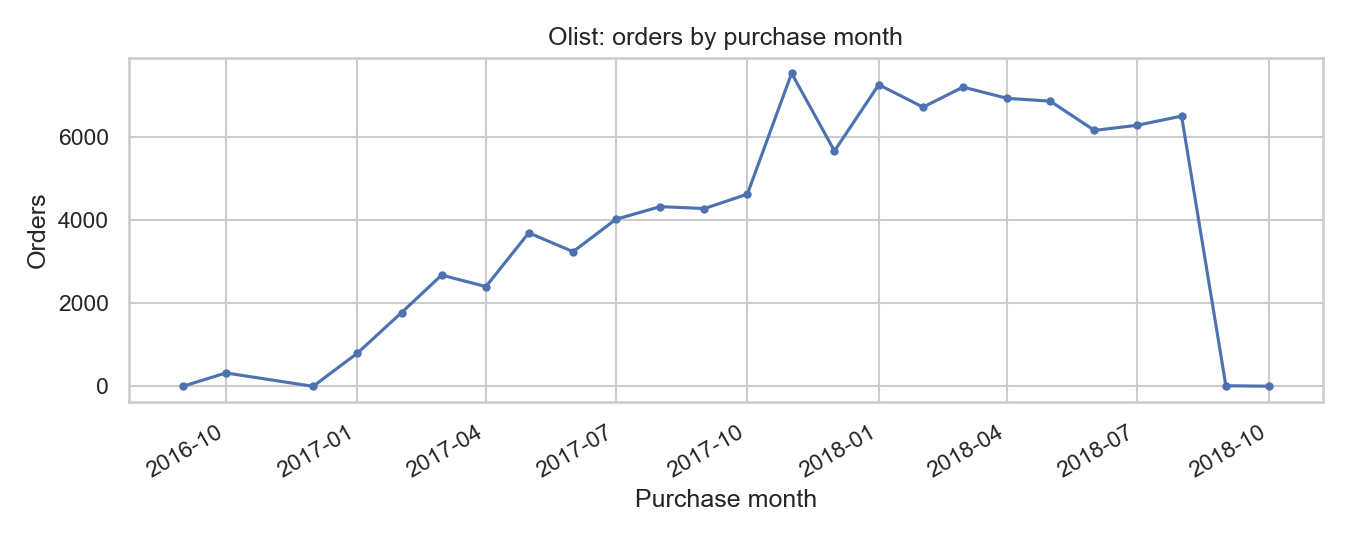
\includegraphics[width=0.86\textwidth]{fig_olist_orders_monthly.png}
\caption{Olist orders by purchase month (measured).}
\label{fig:olist-monthly}
\end{figure}

\begin{figure}[H]\centering
\begin{subfigure}{0.49\textwidth}\centering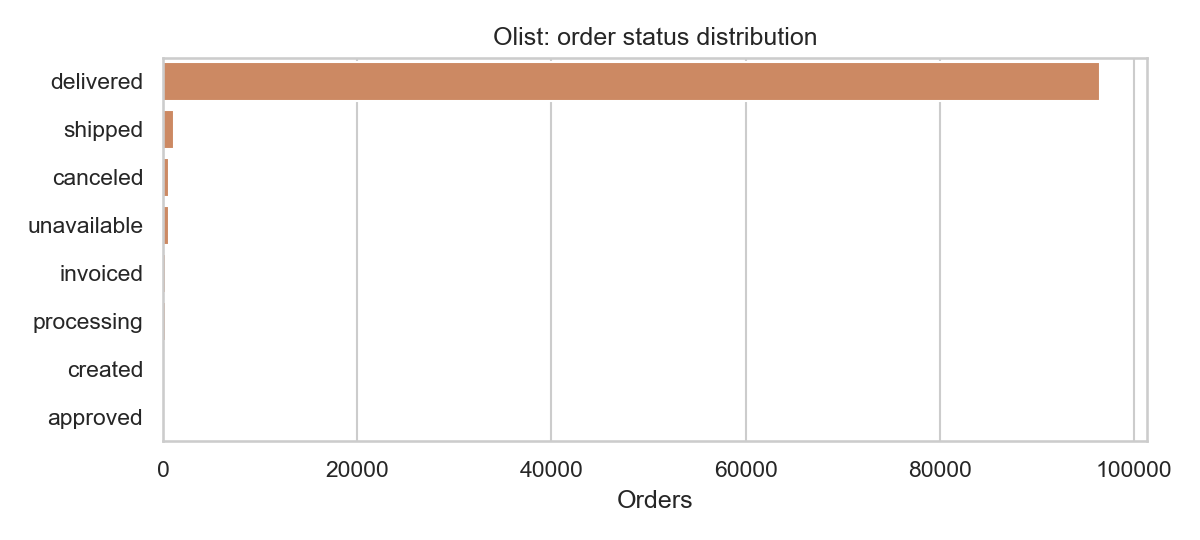
\includegraphics[width=\textwidth]{fig_olist_order_status.png}\caption{Order status.}\end{subfigure}\hfill
\begin{subfigure}{0.49\textwidth}\centering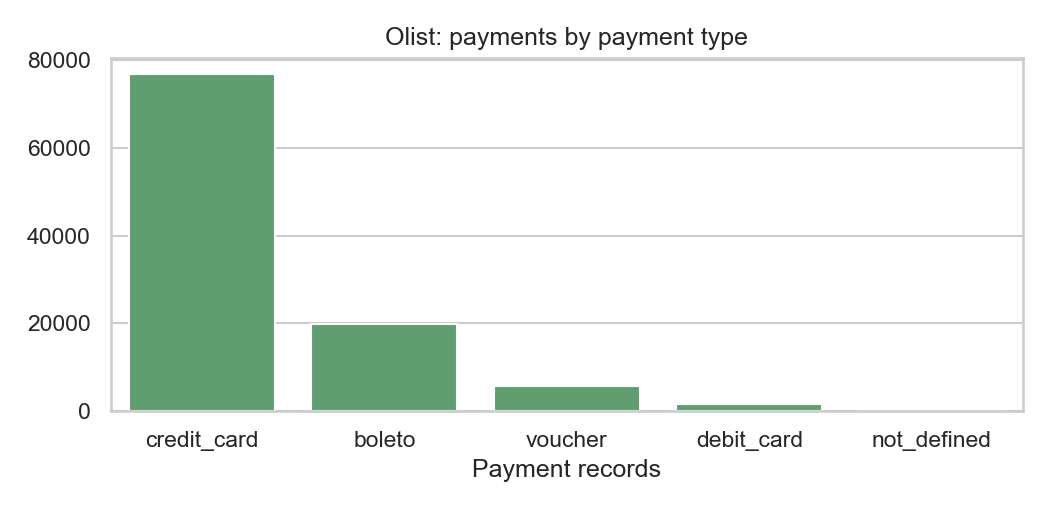
\includegraphics[width=\textwidth]{fig_olist_payment_types.png}\caption{Payment types.}\end{subfigure}
\caption{Olist categorical distributions (measured).}
\label{fig:olist-status}
\end{figure}

\begin{figure}[H]\centering
\begin{subfigure}{0.45\textwidth}\centering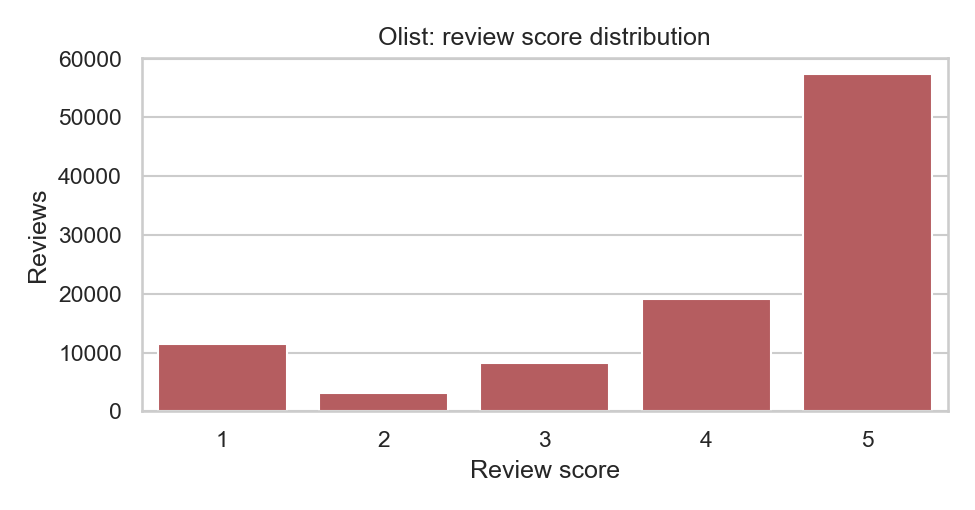
\includegraphics[width=\textwidth]{fig_olist_review_scores.png}\caption{Review scores.}\end{subfigure}\hfill
\begin{subfigure}{0.53\textwidth}\centering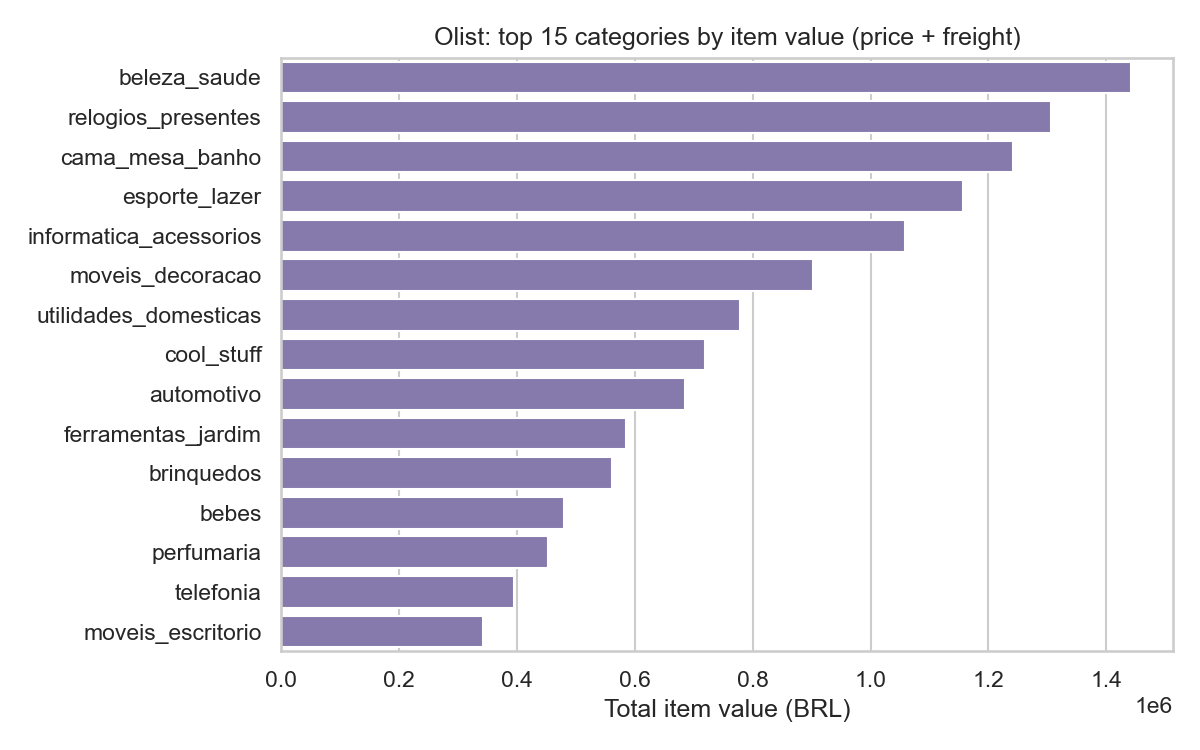
\includegraphics[width=\textwidth]{fig_olist_category_revenue.png}\caption{Top categories by item value.}\end{subfigure}
\caption{Olist review scores and top product categories by item value (price + freight), measured.}
\label{fig:olist-reviews}
\end{figure}

\subsection{Olist: monetary and temporal integrity}
Item-level monetary totals are: prices 13{,}591{,}643.70 BRL; freight 2{,}251{,}909.54 BRL; combined 15{,}843{,}553.24 BRL. Payment totals are 16{,}008{,}872.12 BRL with a mean payment of 154.10 BRL. There are no zero or negative item prices or freight values. Item price has mean 120.65, median 74.99 and maximum 6{,}735.00 BRL; \code{payment\_value} has maximum 13{,}664.10 BRL and \code{payment\_installments} ranges from 0 to 24.

A simple order-level reconciliation proxy compared the summed item value (price + freight) against the summed payment value for the 98{,}665 orders that have both. In 98{,}287 orders (99.62\%) the two totals agree within one cent; the mean absolute difference is 0.0332 BRL. This is a strong consistency signal and a natural basis for an accounting reconciliation rule.

Temporal ordering checks found \emph{no} orders approved before purchase and \emph{no} orders delivered before purchase, but 23 orders recorded as delivered to the customer \emph{before} being handed to the carrier --- a small candidate data-quality anomaly worth flagging. Product-category translation coverage is high: 32{,}328 of 32{,}341 categorised products (99.96\%) have an English translation (the translation file has 71 rows).

\subsection{Online Retail II: completeness, duplicates and business signals}
Table~\ref{tab:retail-quality} summarises the two sheets (and, where useful, their combination). Both sheets share the same eight columns. The most consequential completeness issue is the missing \code{Customer ID}: 20.54\% of lines in 2009--2010 and 24.93\% in 2010--2011 (22.77\% overall). The \code{Description} field is missing for a small fraction of lines (0.56\% and 0.27\%). Exact duplicate rows occur in both sheets (6{,}865 and 5{,}268 raw duplicates); because normalisation only reformats codes, the cleaned duplicate counts match the raw counts, confirming the duplicates are genuine repeated source lines rather than artefacts of cleaning.

Cancellations are encoded by an invoice number beginning with \code{C}. There are 4{,}592 cancellation invoices in 2009--2010 and 3{,}836 in 2010--2011 (8{,}292 combined). Negative quantities occur on 12{,}326 and 10{,}624 lines respectively; most coincide with cancellation invoices, but 2{,}121 and 1{,}336 lines respectively have a negative quantity on a \emph{non}-cancellation invoice (adjustments). Zero prices occur on 3{,}687 and 2{,}515 lines, and there are a handful of negative prices (3 and 2 lines). Extreme quantities are present (minimum $-80{,}995$ and maximum $80{,}995$ in 2010--2011), consistent with stock adjustments or data-entry issues rather than ordinary sales.

\begin{table}[H]
\centering
\small
\caption{Online Retail II per-sheet quality and business signals (measured).}
\label{tab:retail-quality}
\begin{tabular}{lrr}
\toprule
\textbf{Metric} & \textbf{2009-2010} & \textbf{2010-2011} \\
\midrule
Rows & 525{,}461 & 541{,}910 \\
Distinct invoices & 28{,}816 & 25{,}900 \\
Cancellation invoices & 4{,}592 & 3{,}836 \\
Cancellation rows & 10{,}206 & 9{,}288 \\
Distinct stock codes & 4{,}631 & 4{,}070 \\
Negative-quantity rows & 12{,}326 & 10{,}624 \\
Negative qty, non-cancellation & 2{,}121 & 1{,}336 \\
Zero-price rows & 3{,}687 & 2{,}515 \\
Negative-price rows & 3 & 2 \\
Missing \code{Customer ID} (\%) & 20.54 & 24.93 \\
Distinct customers & 4{,}383 & 4{,}372 \\
Distinct countries & 40 & 38 \\
Exact duplicate rows (raw) & 6{,}865 & 5{,}268 \\
Date range (min--max) & 2009-12-01 -- 2010-12-09 & 2010-12-01 -- 2011-12-09 \\
Net revenue (\pounds) & 9{,}539{,}480 & 9{,}747{,}770 \\
Gross positive lines (\pounds) & 10{,}306{,}300 & 10{,}666{,}700 \\
Value of negative lines (\pounds) & $-766{,}781$ & $-918{,}937$ \\
\bottomrule
\end{tabular}
\end{table}

Combined across the two sheets: 1{,}067{,}371 lines, 53{,}628 distinct invoices, 5{,}942 distinct customers, 5{,}304 distinct stock codes and 43 countries; net revenue is 19{,}287{,}250.57 \pounds. Of the customers, 2{,}813 appear in both periods, 1{,}570 only in 2009--2010 and 1{,}559 only in 2010--2011, so the two sheets are neither disjoint nor identical. For positive lines, the median line value is 9.96 \pounds, the 95th percentile 60.00 \pounds, the 99th percentile 183.60 \pounds and the maximum 168{,}469.60 \pounds --- a heavily right-skewed distribution.

\paragraph{Interpretation.} Negative quantities, zero or negative prices, cancellations and very large-magnitude quantities are best understood as a mixture of legitimate business processes (returns, cancellations, adjustments, wholesale orders) and possible data-entry issues. They are \emph{candidate} signals; the dataset contains no verified fraud outcome labels, so these patterns are not evidence of fraud.

Figures~\ref{fig:retail-monthly}--\ref{fig:retail-more} visualise the monthly activity, revenue, country concentration, value distribution, per-period signals and cancellation rate. Sales peak in November in both periods, consistent with holiday-season wholesale ordering, and the United Kingdom dominates (92.46\% of lines in 2009--2010).

\begin{figure}[H]\centering
\begin{subfigure}{0.49\textwidth}\centering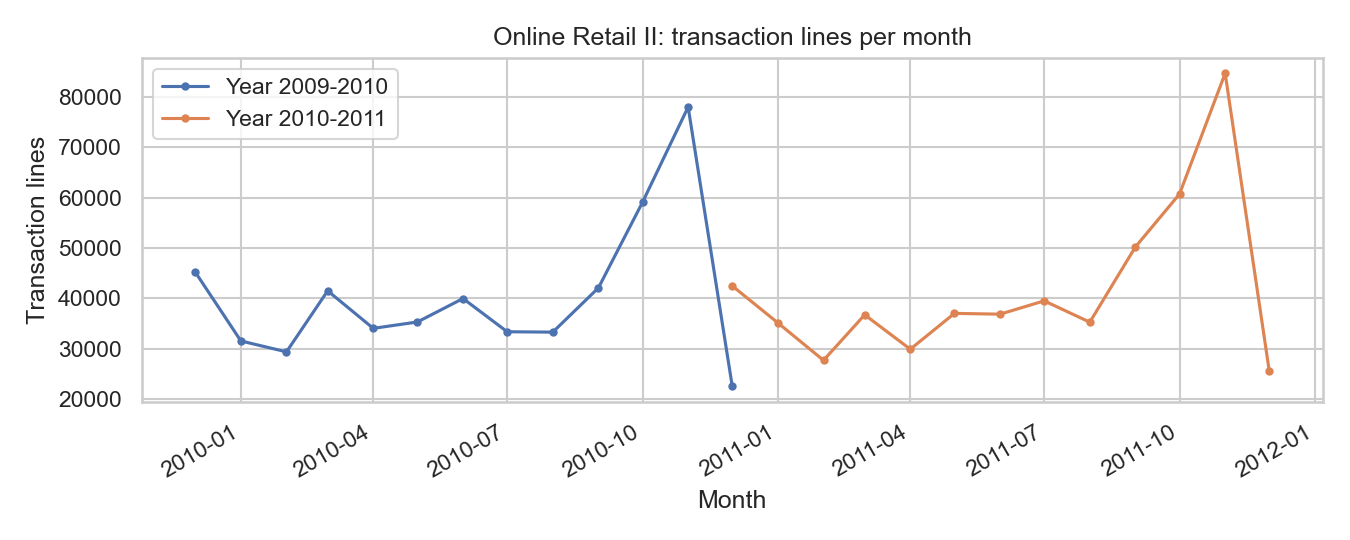
\includegraphics[width=\textwidth]{fig_retail_monthly_lines.png}\caption{Lines per month.}\end{subfigure}\hfill
\begin{subfigure}{0.49\textwidth}\centering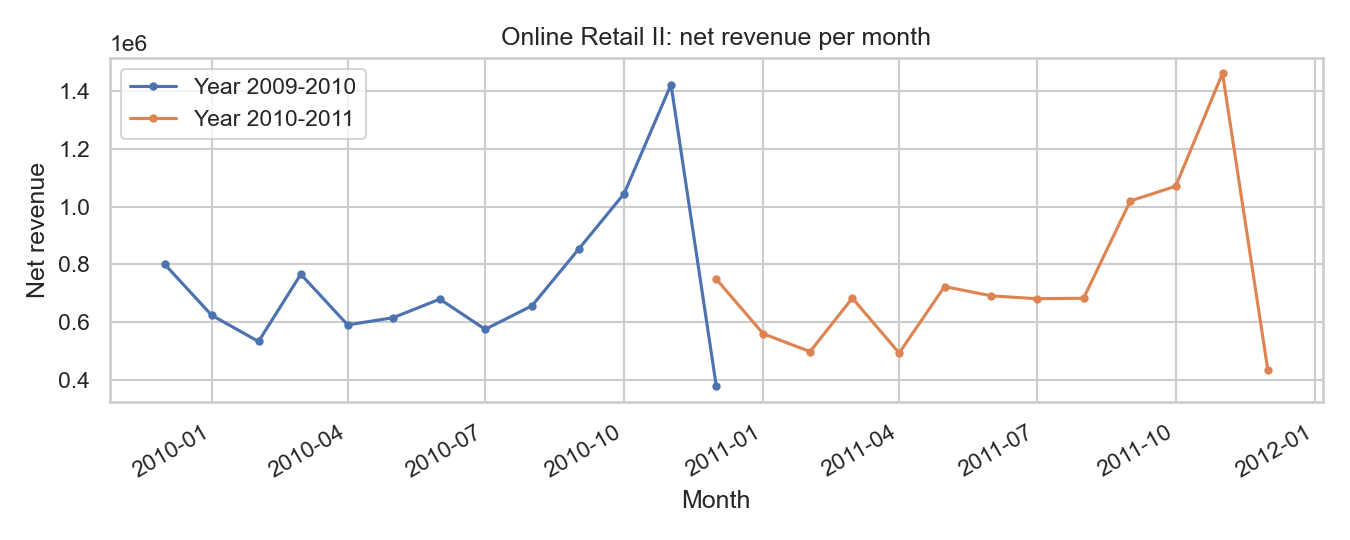
\includegraphics[width=\textwidth]{fig_retail_net_revenue_monthly.png}\caption{Net revenue per month.}\end{subfigure}
\caption{Online Retail II monthly activity (measured).}
\label{fig:retail-monthly}
\end{figure}

\begin{figure}[H]\centering
\begin{subfigure}{0.49\textwidth}\centering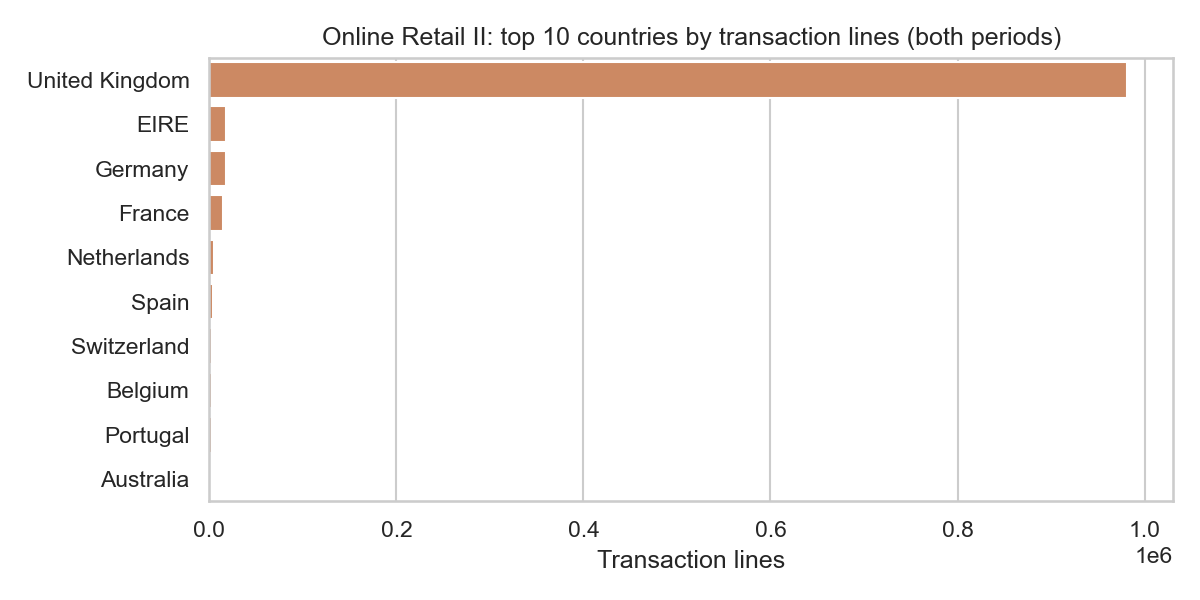
\includegraphics[width=\textwidth]{fig_retail_top_countries.png}\caption{Top countries.}\end{subfigure}\hfill
\begin{subfigure}{0.49\textwidth}\centering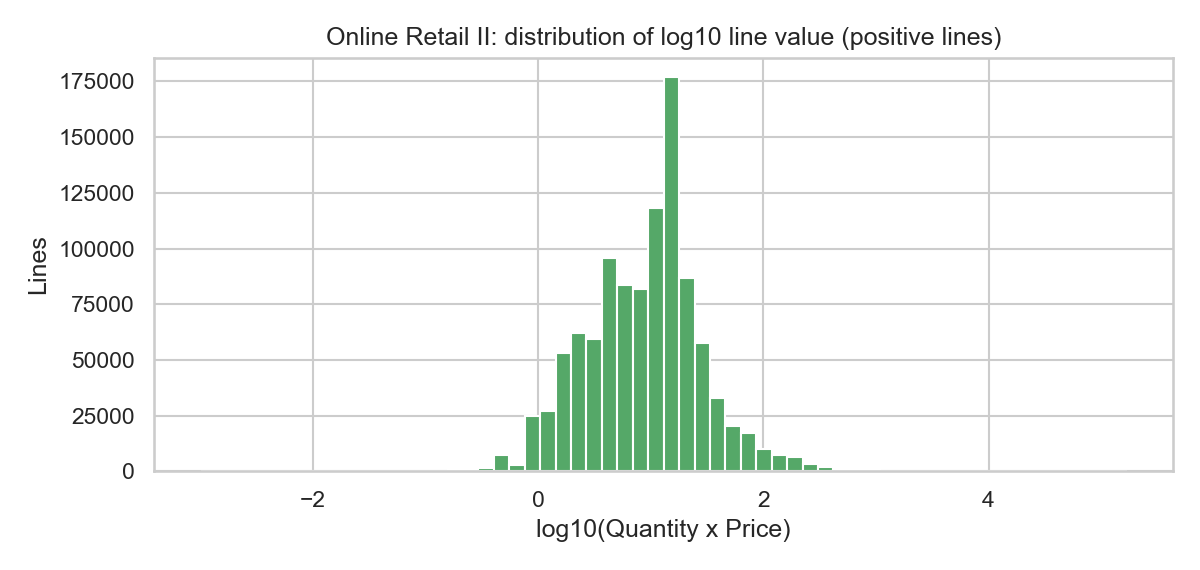
\includegraphics[width=\textwidth]{fig_retail_value_distribution.png}\caption{Line-value distribution.}\end{subfigure}
\caption{Online Retail II country concentration and value distribution (measured).}
\label{fig:retail-dist}
\end{figure}

\begin{figure}[H]\centering
\begin{subfigure}{0.49\textwidth}\centering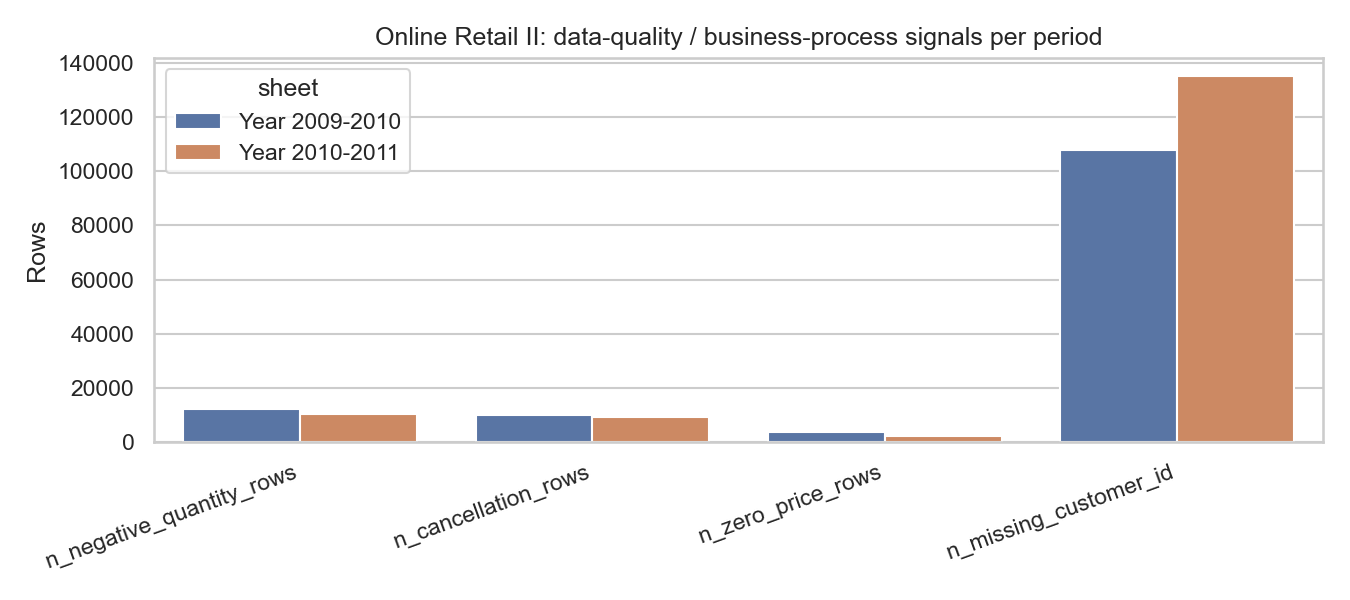
\includegraphics[width=\textwidth]{fig_retail_quality_signals.png}\caption{Quality signals per period.}\end{subfigure}\hfill
\begin{subfigure}{0.49\textwidth}\centering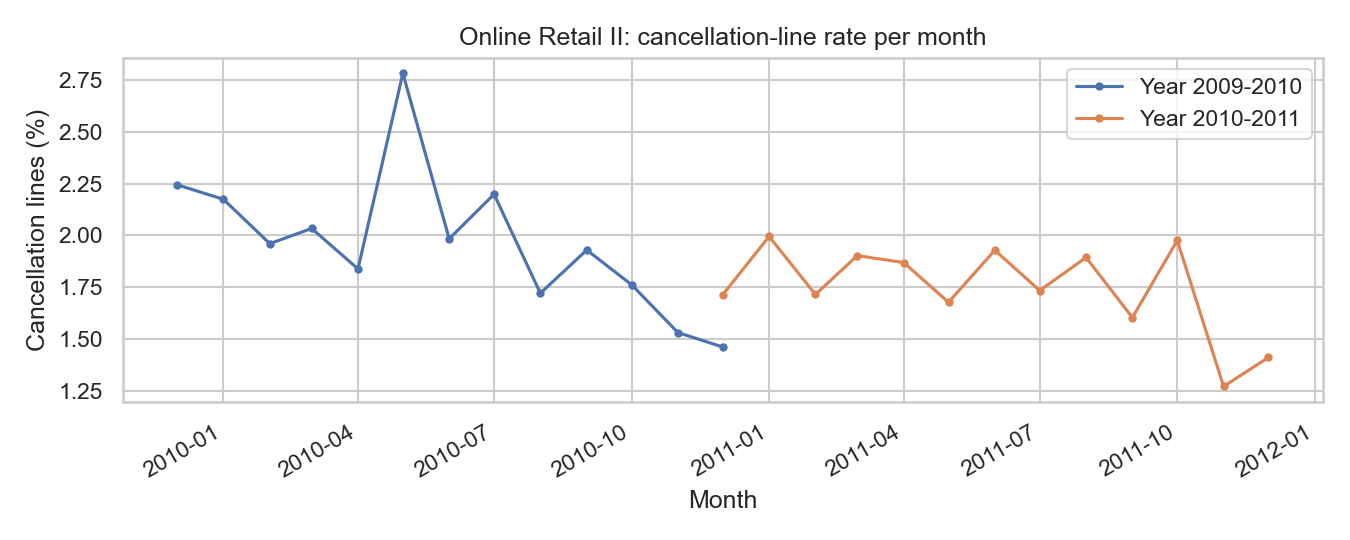
\includegraphics[width=\textwidth]{fig_retail_cancellation_rate.png}\caption{Cancellation rate per month.}\end{subfigure}
\caption{Online Retail II quality signals and cancellation rate (measured).}
\label{fig:retail-more}
\end{figure}

% ===========================================================================
\section{Data Quality Assessment}
% ===========================================================================
Figure~\ref{fig:completeness} contrasts the highest-missing columns of both datasets. The Olist dataset is nearly complete in its structural columns and its missingness is explainable by business status (undelivered orders) or optional free text. Online Retail II's missing \code{Customer ID} is structural: anonymous transactions (22.77\% overall) cannot be attributed to a customer, which limits customer-level analyses but does not prevent transaction-level analysis.

\begin{figure}[H]\centering
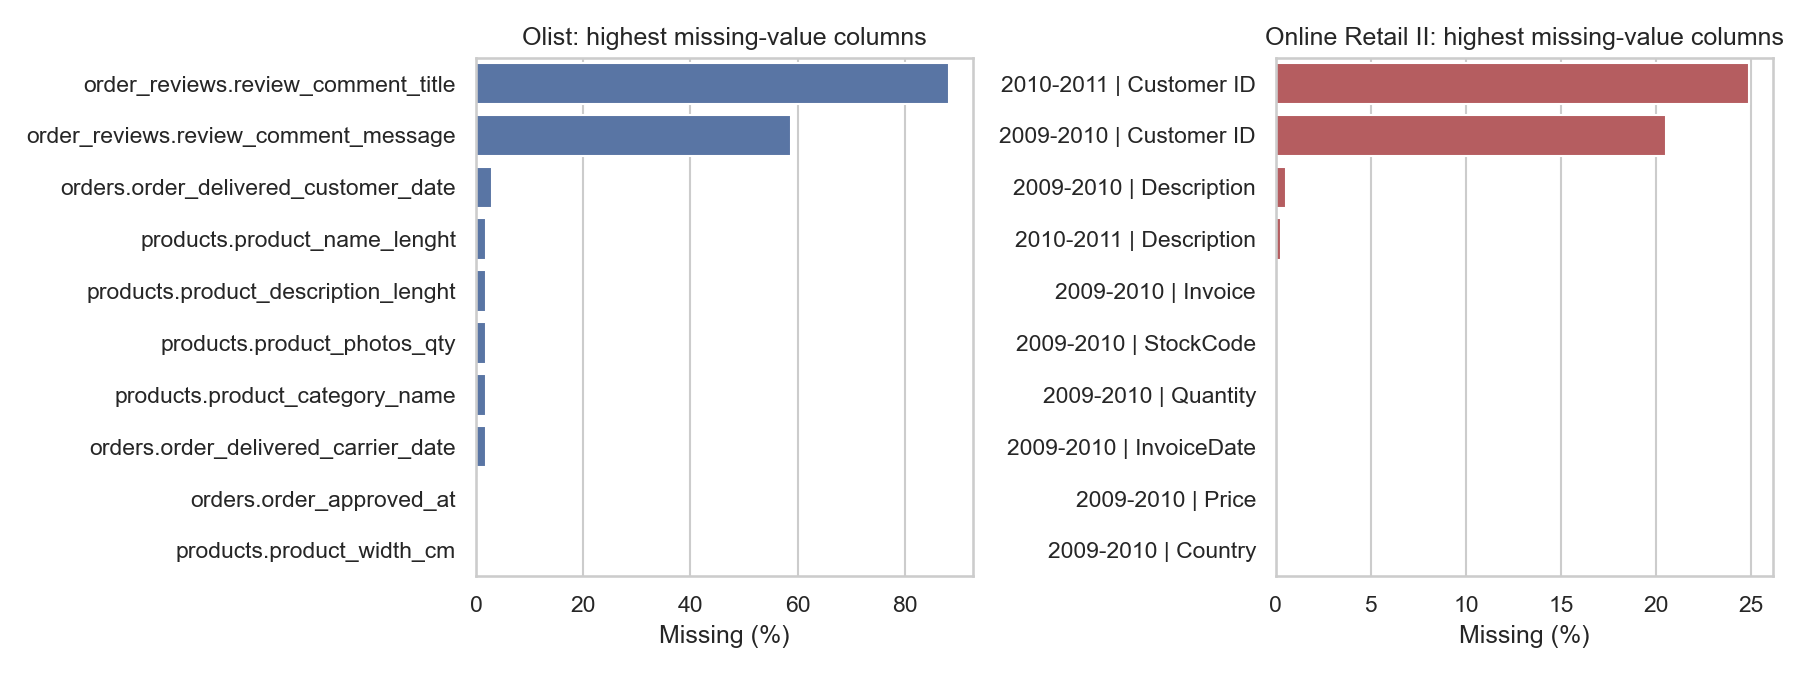
\includegraphics[width=0.95\textwidth]{fig_completeness_comparison.png}
\caption{Completeness comparison: highest missing-value columns in each dataset (measured).}
\label{fig:completeness}
\end{figure}

\paragraph{Summary of quality findings.}
\begin{itemize}
\item \textbf{Olist:} clean keys, full referential integrity, explainable missingness, small temporal inconsistencies (23 orders), heavy but meaningful duplicate geolocation rows (26.18\%), no returns/refunds table and no cost or margin data.
\item \textbf{Online Retail II:} no relational schema, 22.77\% missing customer identifiers, genuine repeated lines, cancellations and adjustments encoded in-band, extreme quantities and a few negative prices, but a rich, well-defined monetary structure and a two-year observation window.
\end{itemize}

% ===========================================================================
\section{Comparative Analysis}
% ===========================================================================
Table~\ref{tab:comparison} compares the two datasets against the project's selection criteria. The comparison mixes measured facts (rows, columns, missingness, date ranges, monetary totals) with qualitative judgements that are grounded in those facts; the qualitative cells are explicitly interpretive.

\begin{longtable}{L{3.1cm}L{6.0cm}L{6.0cm}}
\caption{Comparative analysis of the Olist and Online Retail II datasets.}\label{tab:comparison}\\
\toprule
\textbf{Criterion} & \textbf{Olist} & \textbf{Online Retail II} \\
\midrule
\endfirsthead
\toprule
\textbf{Criterion} & \textbf{Olist} & \textbf{Online Retail II} \\
\midrule
\endhead
\footnotesize
Domain & Brazilian online marketplace (multiple sellers) & UK-based online wholesaler of gift-ware \\
Provenance & Kaggle distribution; nine relational CSVs; CC BY-NC-SA 4.0 & UCI ML Repository, Chen (2012); one workbook, two sheets; CC BY 4.0 \\
Time coverage & 2016-09-04 to 2018-10-17 (purchase dates) & 2009-12-01 to 2011-12-09 \\
Structure & 9 files, 1{,}550{,}922 rows, 52 columns; normalised & 2 sheets, 1{,}067{,}371 rows, 8 columns; denormalised fact table \\
Granularity & order, order item, payment, review, product, seller & one row per invoice line \\
Main entities & customers, orders, items, payments, reviews, products, sellers, geolocation & invoice, stock code, quantity, price, date, customer, country \\
Missingness & structural (undelivered timestamps); optional review text; 1.85\% product metadata & 22.77\% missing \code{Customer ID}; 0.28--0.56\% missing description \\
Duplicates & negligible except geolocation (26.18\%) & repeated invoice lines (raw = cleaned) \\
Key concerns & category translation, timestamp gaps & mixed-type codes, cancellations, negatives \\
E-commerce use & strong: lifecycle, status, payments, reviews, multi-seller & strong: transaction sales, countries, repeat customers \\
Inventory use & indirect demand analysis only; no stock levels & indirect demand analysis only; no stock levels \\
Accounting use & reconciliation proxies (99.62\% agreement) & line-value revenue, cancellations, adjustments \\
Anomaly use & temporal, price, delivery and review anomalies & negative qty, zero/neg.\ price, extreme values \\
Governance/audit use & multi-table evidence retrieval and traceability & transaction-level rule checks and trails \\
Limitations & no returns/refunds, cost or stock data & no product master, order status or cost data; no labels \\
\bottomrule
\end{longtable}

\paragraph{Strengths and weaknesses.}
\emph{Olist} is structurally the richer dataset for a governed multi-agent research prototype: its normalised schema, clean keys and full referential integrity make it easy to implement multi-step workflows, cross-entity validation and evidence retrieval, and its order-level payment reconciliation signal (99.62\% within one cent) is directly useful for the Accounting agent. Its weaknesses are the absence of returns/refunds, cost or inventory data, and the geolocation duplication. \emph{Online Retail II} offers a materially longer window and larger transaction volume with explicit cancellations and adjustments, which is valuable for the Risk/Anomaly agent and for revenue analysis, but its lack of relational structure and the 22.77\% missing customer identifiers limit customer-centric and inventory analyses.

\paragraph{Recommendation.}
Conditional on the evidence above, we recommend \textbf{Olist as the primary dataset} for multi-table e-commerce workflows, accounting reconciliation prototypes and audit experiments, and \textbf{Online Retail II as the complementary dataset} for transaction-level anomaly-detection and revenue/cancellation analysis. The two datasets should \textbf{not} be merged into a single artificial dataset: they differ in currency (BRL vs.\ \pounds), period, schema and semantics, and any merge would fabricate relationships that do not exist. They should be ingested through separate adapters into independent pipelines, optionally normalised into a common internal event representation only for the specific fields where a defensible mapping exists.

% ===========================================================================
\section{Mapping Datasets to the Proposed Agents}
% ===========================================================================
Table~\ref{tab:agents} maps each proposed agent to the evidence available in the datasets, the tasks that can be implemented, example questions, evaluation metrics and the most important limitations. A recurring theme is the distinction between what the \emph{data} provide and what the \emph{prototype} must generate: audit logs, policy decisions and multi-agent workflows are prototype artefacts, not dataset contents.

\begin{longtable}{L{2.2cm}L{3.6cm}L{4.0cm}L{5.2cm}}
\caption{Mapping of proposed agents to available data and research tasks.}\label{tab:agents}\\
\toprule
\textbf{Agent} & \textbf{Relevant data} & \textbf{Implementable tasks} & \textbf{Key limitations} \\
\midrule
\endfirsthead
\toprule
\textbf{Agent} & \textbf{Relevant data} & \textbf{Implementable tasks} & \textbf{Key limitations} \\
\midrule
\endhead
\footnotesize
Orchestrator / Coordination &
Olist orders, items, payments, reviews joined by \code{order\_id}; Retail invoice lines ordered by date &
Simulate multi-step order workflows with explicit dependencies (approve $\rightarrow$ pick/pack $\rightarrow$ ship $\rightarrow$ invoice $\rightarrow$ reconcile); measure outcomes &
Dataset structure alone does not demonstrate coordination; workflow behaviour must come from the prototype \\
E-Commerce &
Olist \code{order\_status}, timestamps, payments, reviews; Retail invoice, quantity, price, date, country &
Order/transaction analysis, status tracking, sales reporting, cancellation analysis &
Olist has no acquisition/session data; Retail has no order-status concept \\
Inventory &
Olist order items and product attributes; Retail stock code and quantity &
Indirect demand analysis, product velocity ranking, stock-out proxies &
Neither dataset contains real-time stock levels, warehouse history, replenishment events or stock movements \\
Accounting &
Olist payments, item price/freight; Retail line value, cancellations, adjustments &
Reconciliation prototypes, transaction consistency checks, revenue aggregation &
No general ledger, journal entries, tax records or audited statements; Olist reconciliation is item-vs-payment only \\
Risk / Anomaly &
Olist delivery/price/review outliers; Retail negative quantities, zero/negative prices, extreme values &
Transparent rule-based and statistical anomaly flagging; severity scoring &
No ground-truth fraud labels; flagged cases are candidate anomalies, not verified fraud \\
Governance &
Structured fields usable as policy inputs (e.g.\ freight ratio, price $>0$, quantity limits) &
Policy-enforcement prototype with explicitly defined experimental rules; block/escalate decisions &
Datasets contain no governance policies, user permissions or approval workflows \\
Audit &
Business records usable as evidence references &
Record agent actions, timestamps, policy decisions, evidence references and outcomes during experiments &
Audit logs are generated by the prototype, not present in the datasets \\
\bottomrule
\end{longtable}

% ===========================================================================
\section{Proposed Architecture and Data Ingestion Strategy}
% ===========================================================================
\subsection{Layered architecture}
We propose a four-layer prototype:
\begin{enumerate}
\item \textbf{Ingestion and validation layer.} Dataset-specific adapters read the raw files read-only, validate schemas, parse timestamps, preserve missing values and emit a validation report (row counts, key checks, orphan counts). This layer corresponds directly to the analysis package delivered with this report.
\item \textbf{Canonical event layer.} A minimal, justified internal representation for the entities that clearly map across sources: \code{order/transaction}, \code{line item}, \code{payment}, and \code{review/cancellation}. Fields that do not map defensibly (e.g.\ inventory levels, tax) are simply not represented, rather than approximated.
\item \textbf{Agent layer.} The seven agents operate over the canonical events and the dataset-specific stores through explicit interfaces.
\item \textbf{Governance and audit layer.} Every agent action is wrapped by a policy check and an append-only audit event writer.
\end{enumerate}

\subsection{Dataset-specific adapters}
Rather than forcing both datasets into one artificial schema, we keep two adapters:
\begin{itemize}
\item \textbf{Olist adapter:} joins \code{orders} to \code{order\_items}, \code{order\_payments} and \code{order\_reviews} with explicit aggregation to avoid the row inflation measured in Table~\ref{tab:olist-joins}; retains \code{customer\_id}/\code{customer\_unique\_id} as pseudonymous keys.
\item \textbf{Online Retail II adapter:} treats each row as a transaction line; derives an invoice-level view by aggregation; classifies invoices as normal or cancellation using the \code{C} prefix; flags negative quantities, zero/negative prices and extreme values as reviewable signals.
\end{itemize}

\subsection{Minimal common internal representation}
A common representation is justified only for the three concepts present in both sources: a \emph{monetary transaction line} (source, identifier, timestamp, amount, sign, currency), a \emph{payment/settlement} record (Olist only, kept source-specific), and an \emph{exception/cancellation} record. Every canonical field carries a mandatory \code{source} attribute so that evidence traceability is preserved and no meaning is lost.

% ===========================================================================
\section{Example Experimental Scenarios}
% ===========================================================================
Table~\ref{tab:scenarios} gives concrete, reproducible scenarios drawn from the measured data. They are proposals for the prototype, not results.

\begin{table}[H]
\centering
\small
\caption{Proposed experimental scenarios and the metrics they exercise.}
\label{tab:scenarios}
\begin{tabular}{L{3.6cm}L{6.4cm}L{4.6cm}}
\toprule
\textbf{Scenario} & \textbf{Description} & \textbf{Metrics exercised} \\
\midrule
Order reconciliation & For Olist orders with items and payments, the Accounting agent reconciles summed item value against payment value; the Governance agent reviews mismatches beyond a threshold & Reconciliation mismatch rate; policy violation rate \\
Delivery-delay anomaly & The Risk agent flags orders whose delivery exceeded the estimate by a robust threshold; the Audit agent records evidence & Flag rate; evidence traceability \\
Cancellation review & The Risk agent flags Online Retail II lines with negative quantity on non-cancellation invoices and zero/negative prices & Signal rate per rule \\
Demand ranking & The Inventory agent ranks products by sold quantity (Olist items; Retail lines) and flags high-variance products & Ranking stability; coverage \\
Policy enforcement & The Governance agent applies explicit rules (e.g.\ maximum freight-to-price ratio) and blocks or escalates & Violation detection rate; false-block rate \\
End-to-end audit & The Orchestrator runs a multi-agent workflow and the Audit agent reconstructs the decision chain from the event log & Audit coverage; traceability; completion rate \\
\bottomrule
\end{tabular}
\end{table}

% ===========================================================================
\section{Evaluation Protocol and Metrics}
% ===========================================================================
Table~\ref{tab:metrics} classifies the candidate metrics by whether they can be computed \emph{immediately from the datasets} or require the prototype, annotations, synthetic scenarios or external ground truth. This separation prevents over-claiming.

\begin{table}[H]
\centering
\small
\caption{Evaluation metrics and their data requirements.}
\label{tab:metrics}
\begin{tabular}{L{4.6cm}L{4.2cm}L{5.8cm}}
\toprule
\textbf{Metric} & \textbf{Status} & \textbf{Basis / requirement} \\
\midrule
Data validation error rate & Immediate & From schema and key/integrity checks on the raw data \\
Reconciliation mismatch rate & Immediate (proxy) & Olist item-vs-payment comparison (99.62\% within one cent measured) \\
Record duplication rate & Immediate & Exact-duplicate counts (measured) \\
Anomaly flag rate & Immediate (rules) & Rule-based flags on quantities/prices/timestamps \\
Anomaly precision/recall & Requires labels & Needs trustworthy ground-truth annotations, not present \\
Policy violation detection rate & Requires prototype & Depends on experimental policy definitions \\
False-block rate & Requires prototype & Requires prototype outcomes \\
Audit event coverage & Requires prototype & Measured over generated audit logs \\
Evidence traceability & Requires prototype & Fraction of decisions with resolvable evidence references \\
Workflow completion rate & Requires prototype & Multi-step workflows executed by the orchestrator \\
Execution overhead & Requires prototype & Latency and cost of agent runs \\
\bottomrule
\end{tabular}
\end{table}

\paragraph{Baselines.} We recommend three baselines: (i) a no-agent baseline in which a script performs the same reconciliation and validation checks deterministically; (ii) a single-agent baseline where one agent performs all tasks; and (iii) a rule-only baseline for anomaly detection. These isolate the contribution of coordination and governance from the contribution of the underlying analytics.

\paragraph{Reproducibility requirements.} Fixed random seeds for any stochastic method; version-pinned dependencies; immutable raw files; recorded SHA-256 checksums of input files (produced by the analysis package in \code{analysis\_results/dataset\_inventory.csv}); and machine-readable outputs for every reported number.

% ===========================================================================
\section{Audit Event Schema}
% ===========================================================================
The Audit agent must record the prototype's own behaviour. Table~\ref{tab:audit} proposes an append-only audit event schema. Crucially, these events are \emph{generated by the prototype}; they are not attributes of either dataset.

\begin{table}[H]
\centering
\small
\caption{Proposed audit event schema (prototype-generated).}
\label{tab:audit}
\begin{tabular}{L{3.4cm}L{5.0cm}L{6.0cm}}
\toprule
\textbf{Field} & \textbf{Type} & \textbf{Meaning} \\
\midrule
\code{event\_id} & string (UUID) & Unique identifier of the audit event \\
\code{timestamp} & datetime & When the action occurred \\
\code{agent} & string & Agent that acted \\
\code{action} & string & Operation performed \\
\code{policy\_id} & string & Experimental governance rule evaluated \\
\code{policy\_decision} & enum & allow / block / escalate \\
\code{evidence\_refs} & list & Source records (table + key) used as evidence \\
\code{input\_digest} & string (hash) & Hash of the input records \\
\code{outcome} & enum & success / failure / pending \\
\code{notes} & string & Free-text rationale (no personal data) \\
\bottomrule
\end{tabular}
\end{table}

% ===========================================================================
\section{Limitations, Ethical Considerations and Threats to Validity}
% ===========================================================================
\subsection*{Limitations of the datasets}
Neither dataset contains inventory stock levels, replenishment events, stock movements, a general ledger, journal entries, tax records, audited financial statements, governance policies, user permissions, approval workflows or ground-truth fraud labels. Historical business data alone cannot validate the complete operation of a governed multi-agent system: the datasets can supply evidence and evaluation inputs, but the agents, coordination, governance and audit mechanisms must be implemented and evaluated by the prototype.

\subsection*{Ethical considerations and privacy}
Both datasets are anonymised or pseudonymised public releases, but they still describe real commercial behaviour and, in the case of Online Retail II, real customers. We therefore: (i) never reproduce personal identifiers in report tables, figures or examples; (ii) treat free-text review comments as potentially sensitive and do not quote them; and (iii) design the audit schema to exclude personal data. Any deployment of the prototype should consider data-protection obligations such as the GDPR \cite{gdpr2016}. The Online Retail II licence (CC BY 4.0) and the Olist licence (CC BY-NC-SA 4.0, which forbids commercial use and requires share-alike) must be respected when redistributing data or derived artefacts.

\subsection*{Threats to validity}
\begin{itemize}
\item \textbf{Construct validity:} business signals such as negative quantities may reflect legitimate processes; they are not fraud labels.
\item \textbf{External validity:} both datasets cover specific retailers, regions and periods; conclusions may not generalise.
\item \textbf{Internal validity:} join inflation and duplicate rows, if mishandled, can distort aggregates; the analysis reports join factors explicitly to mitigate this.
\item \textbf{Conclusion validity:} metrics requiring ground truth cannot be computed from these data and are marked as such.
\end{itemize}
The data-quality methodology follows established practice \cite{batini2009}, the FAIR principles guide reuse and citation \cite{wilkinson2016}, anomaly detection terminology follows the standard survey \cite{chandola2009}, and governance concepts are framed with reference to the NIST AI RMF \cite{nistAirmf2023} and ISO/IEC 42001 \cite{iso42001}.

% ===========================================================================
\section{Dataset Recommendation and Conclusion}
% ===========================================================================
\paragraph{Recommendation.}
Use \textbf{Olist as the primary dataset}: its normalised schema, clean keys, full referential integrity and a strong order-level reconciliation signal make it the best foundation for multi-table e-commerce workflows, accounting reconciliation prototypes, governance rules and audit experiments. Use \textbf{Online Retail II as the complementary dataset}: its longer window, larger volume and explicit cancellation/adjustment encoding enrich transaction-level and anomaly-detection work. Keep the two pipelines separate, share only a minimal and explicitly justified common representation, and never merge the sources into one artificial dataset.

\paragraph{Conclusion.}
The exploratory analysis shows that both datasets are usable, real evidence sources with well-understood quality characteristics. Olist is structurally stronger; Online Retail II is temporally and transactionally richer but messier. Neither is sufficient on its own to validate a governed multi-agent system, and neither contains the governance, audit or ground-truth artefacts that the prototype must create. The accompanying analysis package, machine-readable results, figures and tests make the reported findings reproducible and auditable.

% ===========================================================================
% REFERENCES
% ===========================================================================
\bibliographystyle{plain}
\bibliography{references}

% ===========================================================================
% APPENDIX
% ===========================================================================
\appendix
\section{Supplementary Statistics}
\label{app:supp}
\subsection*{A.1 Schema validation}
All nine Olist files and both Online Retail II sheets matched the expected column sets (see \code{analysis\_results/olist\_schema\_validation.csv}). The Online Retail II loader fails fast if the eight expected columns are not present.

\subsection*{A.2 Selected numeric descriptive statistics}
\begin{table}[H]
\centering
\small
\caption{Selected numeric statistics (measured).\label{tab:appendix-num}}
\begin{tabular}{llrrrr}
\toprule
\textbf{Dataset} & \textbf{Column} & \textbf{Mean} & \textbf{Median} & \textbf{Min} & \textbf{Max} \\
\midrule
Olist & \code{price} (BRL) & 120.65 & 74.99 & 0.85 & 6{,}735.00 \\
Olist & \code{freight\_value} (BRL) & 19.99 & 16.26 & 0.00 & 409.68 \\
Olist & \code{payment\_value} (BRL) & 154.10 & 100.00 & 0.00 & 13{,}664.10 \\
Olist & \code{payment\_installments} & 2.85 & 1.00 & 0.00 & 24.00 \\
Olist & \code{review\_score} & 4.09 & 5.00 & 1.00 & 5.00 \\
Retail 2009-2010 & \code{Quantity} & 10.34 & 3.00 & $-9{,}600$ & 19{,}152 \\
Retail 2009-2010 & \code{Price} (\pounds) & 4.69 & 2.10 & $-53{,}594.40$ & 25{,}111.10 \\
Retail 2010-2011 & \code{Quantity} & 9.55 & 3.00 & $-80{,}995$ & 80{,}995 \\
Retail 2010-2011 & \code{Price} (\pounds) & 4.61 & 2.08 & $-11{,}062.10$ & 38{,}970.00 \\
\bottomrule
\end{tabular}
\end{table}

\subsection*{A.3 Machine-readable artefacts}
The following files are produced by \code{python -m analysis} and contain the exact figures cited in this report:
\begin{itemize}\small
\item \path{analysis_results/table_dimensions.csv}, \path{olist_schema_validation.csv}
\item \path{analysis_results/olist_column_profile.csv}, \path{olist_numeric_stats.csv}, \path{olist_categorical_stats.csv}, \path{olist_temporal_profile.csv}
\item \path{analysis_results/olist_primary_key_checks.csv}, \path{olist_referential_integrity.csv}, \path{olist_join_cardinality.csv}, \path{olist_join_expansion.csv}, \path{olist_duplicate_rows.csv}
\item \path{analysis_results/olist_value_counts.csv}, \path{olist_category_revenue.csv}, \path{olist_monthly_orders.csv}
\item \path{analysis_results/retail_column_profile.csv}, \path{retail_numeric_stats.csv}, \path{retail_quality_metrics.csv}, \path{retail_duplicate_rows.csv}, \path{retail_value_counts.csv}, \path{retail_admin_stock_codes.csv}, \path{retail_monthly_activity.csv}
\item \path{analysis_results/dataset_comparison.csv}, \path{agent_suitability.csv}, \path{summary.json}
\end{itemize}

\subsection*{A.4 Tests}
Thirteen unit tests (\code{tests/test\_analysis.py}) verify the metric definitions, including missing-value preservation, duplicate counting, key checks, referential integrity, numeric sign counts, temporal profiling, cancellation detection and revenue definitions. All tests pass.

\end{document}
